\chapter{Reference cells}

In this chapter, a set of standard reference cells are defined.
The following five reference cells are covered by the UFC specification:
\emph{interval},
\emph{triangle},
\emph{quadrilateral},
\emph{tetrahedron},
\emph{hexahedron}.

On each reference cell, an \emph{ad-hoc} ordering is picked for the
vertices of the cell. The ordering of the remaining entities (edges,
faces, \ldots) then follows by a simple rule.

It is assumed that whenever a UFC dof map specifies that entities of a
certain topological dimension are needed, the ordering of those
entities follow the convention defined in this chapter for each cell
in the mesh.

\begin{table}[H]
  \begin{center}
    \begin{tabular}{|l|l|}
      \hline
      Name & Description \\
      \hline
      \hline
      \emph{interval}      & the 1D reference interval \\
      \hline
      \emph{triangle}      & the 2D reference triangle \\
      \hline
      \emph{quadrilateral} & the 2D reference square \\
      \hline
      \emph{tetrahedron}   & the 3D reference tetrahedron \\
      \hline
      \emph{hexahedron}    & the 3D reference cube \\
      \hline
    \end{tabular}
    \caption{Reference cells covered by the UFC specification.}
  \end{center}
\end{table}

\section{Basic concepts}

\subsection{Mesh entities}

The topological entities of a cell (or mesh) are referred to as
\emph{mesh entities}. A mesh entity can be identified with a pair
$(d, i)$, where $d$ is the topological dimension of the mesh entity and $i$
is a unique index of the mesh entity. Mesh entities are numbered
within each topological dimension from $0$ to $n_d-1$, where $n_d$ is
the number of mesh entities of topological dimension $d$.

\subsection{Named mesh entities}

For convenience, mesh entities of topological dimension $0$ are
referred to as \emph{vertices}, entities of dimension $1$
\emph{edges}, entities of dimension $2$ \emph{faces}, entities of
\emph{codimension} $1$ \emph{facets} and entities of codimension $0$
\emph{cells}. These concepts are summarized in
Table~\ref{tab:entities}.

\begin{table}[H]
  \begin{center}
    \begin{tabular}{|l|c|c|}
      \hline
      Entity & Dimension & Codimension \\
      \hline
      Vertex & $0$       & -- \\
      Edge   & $1$       & -- \\
      Face   & $2$       & -- \\
      & & \\
      Facet  & --      &  $1$ \\
      Cell   & --      &  $0$ \\
      \hline
    \end{tabular}
    \caption{Named mesh entities.}
    \label{tab:entities}
  \end{center}
\end{table}

\subsection{Ordering of mesh entities}

On each reference cell, an \emph{ad-hoc} ordering is picked for its
vertices (the mesh entities of topological dimension zero). The
remaining entities are then ordered within each topological dimension
by identifying each entity with the corresponding tuple of
non-incident vertices and then ordering those tuples
lexicographically.

As an illustration, consider the ordering of edges (the mesh entities
of topological dimension one) on a triangle. In
Figure~\ref{fig:orderingexample}, the vertices of the reference
triangle are numbered counter-clockwise in the plane. The edges of the
reference triangle may then be numbered by identifying each edge with
the vertices not incident with that edge. Since there is only one such
vertex for each edge, each edge is identified with the vertex
oppositve to the edge. We thus identify the three edges in the
reference triangle with the tuples $(0)$, $(1)$ and $(2)$
The first of these is edge $e^0$ between vertices $v^1$ and $v^2$
opposite to vertex $v^0$.

Similarly, we identify the six edges of the reference tetrahedron with
the tuples $(0, 1)$, $(0, 2)$, $(0, 3)$, $(1, 2)$, $(1, 3)$ and
$(2, 3)$. The first of these is edge $e^0$ between vertices $v^2$ and
$v^3$ opposite to vertices $v^0$ and $v^1$.

\begin{figure}[H]
  \begin{center}
    \psfrag{v0}{$v^0$}
    \psfrag{v1}{$v^1$}
    \psfrag{v2}{$v^2$}
    \psfrag{e0}{$e^0$}
    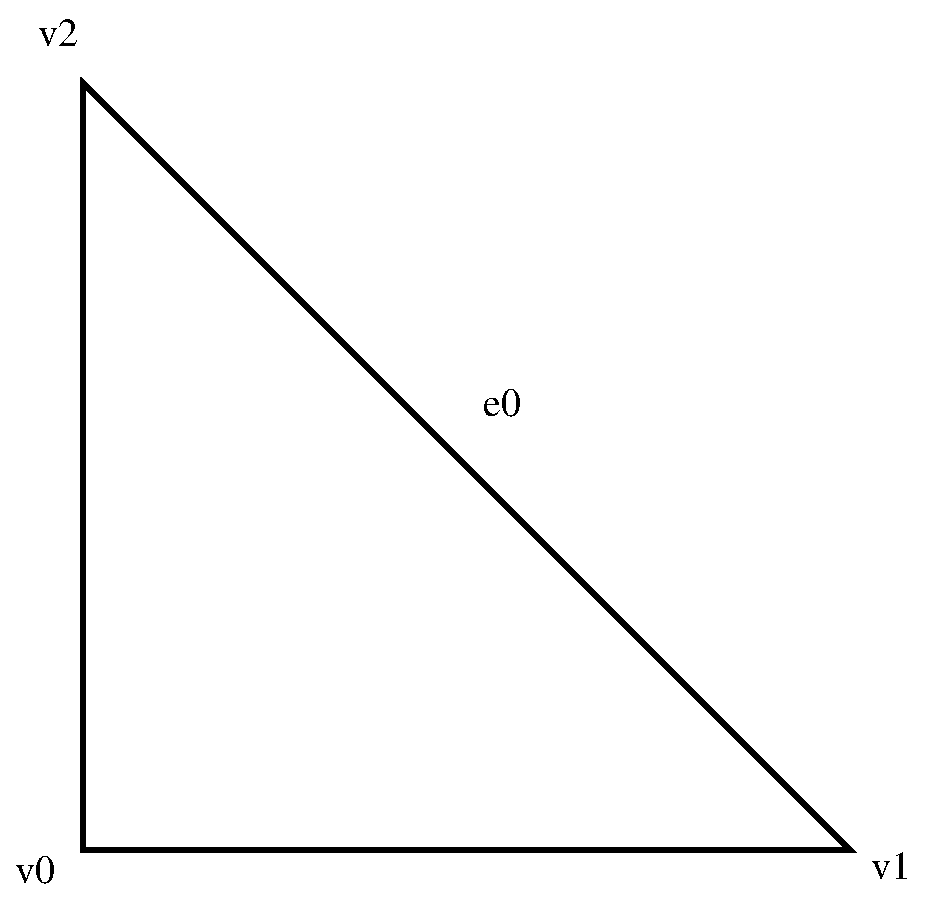
\includegraphics[width=10cm]{eps/ordering_example_triangle.eps}
    \caption{Entities are ordered based on a lexicographical ordering
      of non-incident vertices. The first edge $e^0$ is non-incident
      with vertex $v^0$.}
    \label{fig:orderingexample}
  \end{center}
\end{figure}

\begin{figure}[H]
  \begin{center}
    \psfrag{v0}{$v^0$}
    \psfrag{v1}{$v^1$}
    \psfrag{v2}{$v^2$}
    \psfrag{v3}{$v^3$}
    \psfrag{e0}{$e^0$}
    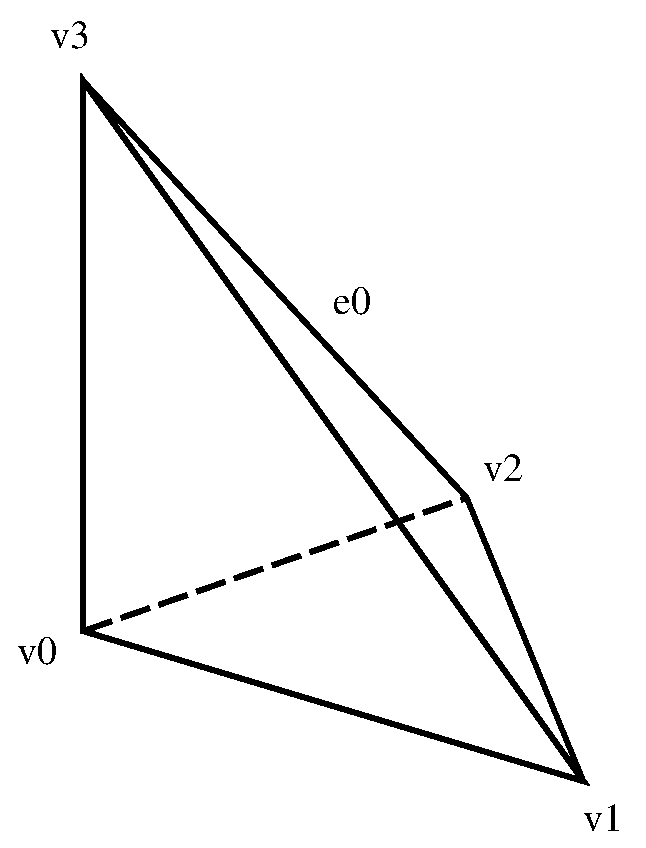
\includegraphics[width=10cm]{eps/ordering_example_tetrahedron.eps}
    \caption{Entities are ordered based on a lexicographical ordering
      of non-incident vertices. The first edge $e^0$ is non-incident
      with vertices $v^0$ and $v^1$.}
    \label{fig:orderingexample}
  \end{center}
\end{figure}

\newpage
\section{The reference interval}

\begin{figure}[H]
  \begin{center}
    \psfrag{0}{$0$}
    \psfrag{1}{$1$}
    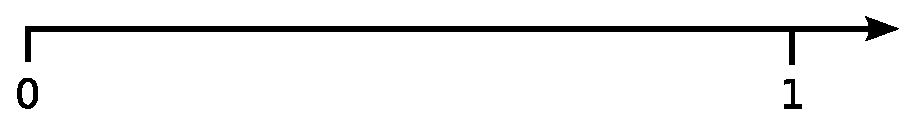
\includegraphics[width=10cm]{eps/interval.eps}
    \caption{The reference interval.}
  \end{center}
\end{figure}

\newpage
\section{The reference triangle}

\begin{figure}[H]
  \begin{center}
    \psfrag{v0}{$(0, 0)$}
    \psfrag{v1}{$(1, 0)$}
    \psfrag{v2}{$(0, 1)$}
    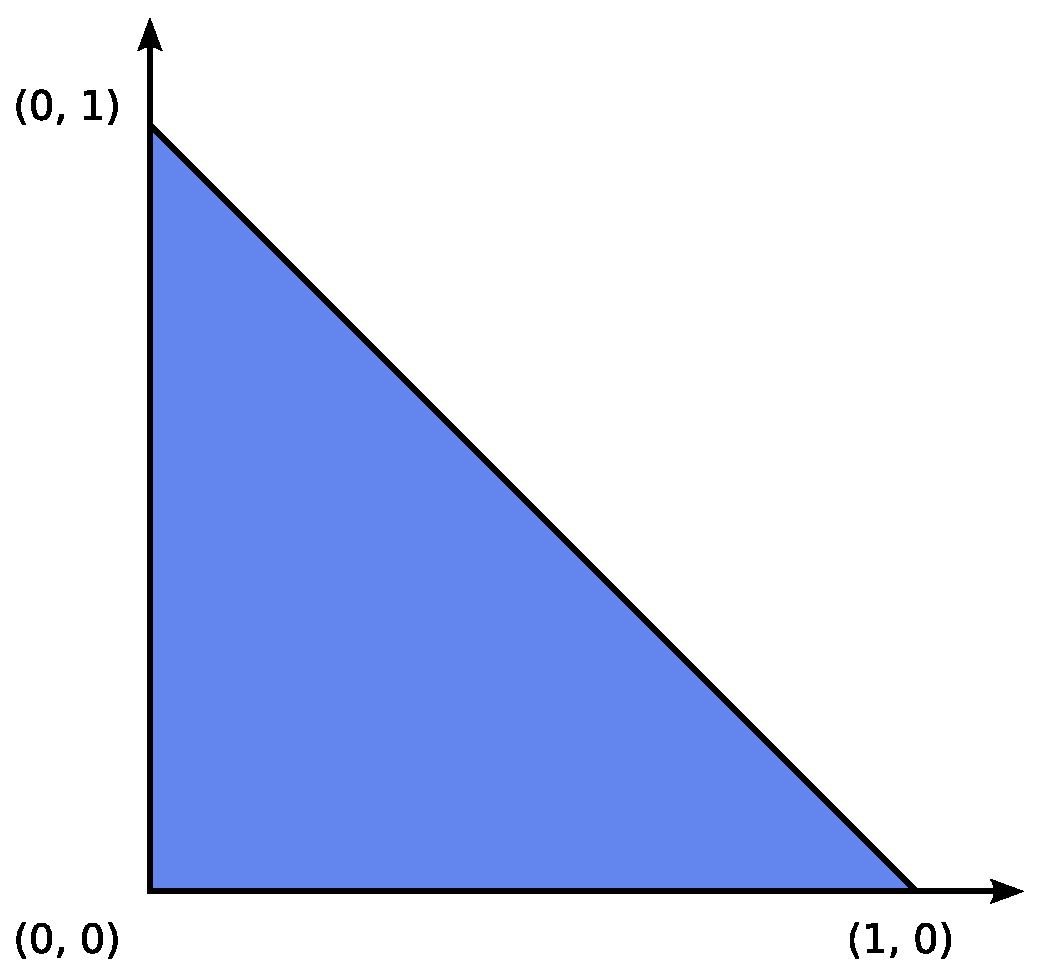
\includegraphics[width=10cm]{eps/triangle.eps}
    \caption{The reference triangle.}
  \end{center}
\end{figure}

\newpage
\section{The reference quadrilateral}

\begin{figure}[H]
  \begin{center}
    \psfrag{v0}{$(0, 0)$}
    \psfrag{v1}{$(1, 0)$}
    \psfrag{v2}{$(1, 1)$}
    \psfrag{v3}{$(0, 1)$}
    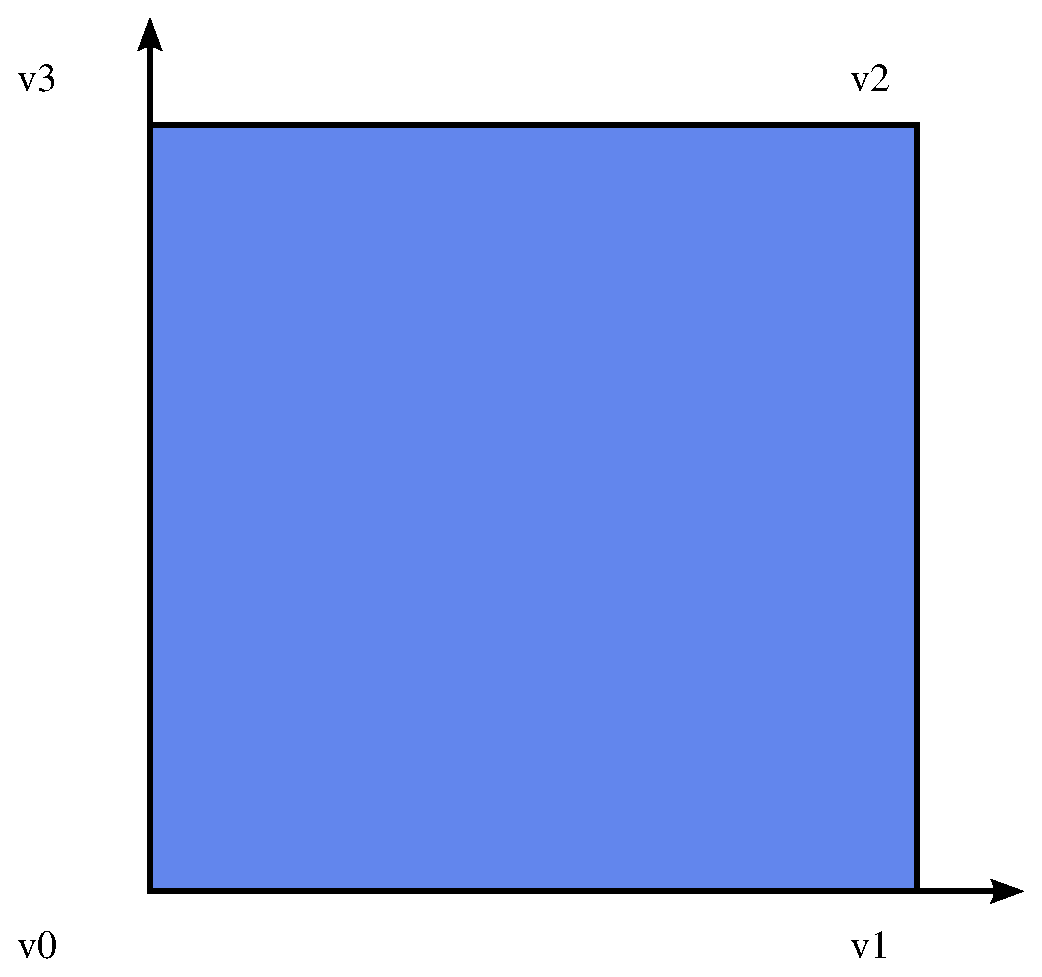
\includegraphics[width=10cm]{eps/quadrilateral.eps}
    \caption{The reference quadrilateral.}
  \end{center}
\end{figure}

\newpage
\section{The reference tetrahedron}

\begin{figure}[H]
  \begin{center}
    \psfrag{v0}{$(0, 0, 0)$}
    \psfrag{v1}{$(1, 0, 0)$}
    \psfrag{v2}{$(0, 1, 0)$}
    \psfrag{v3}{$(0, 0, 1)$}
    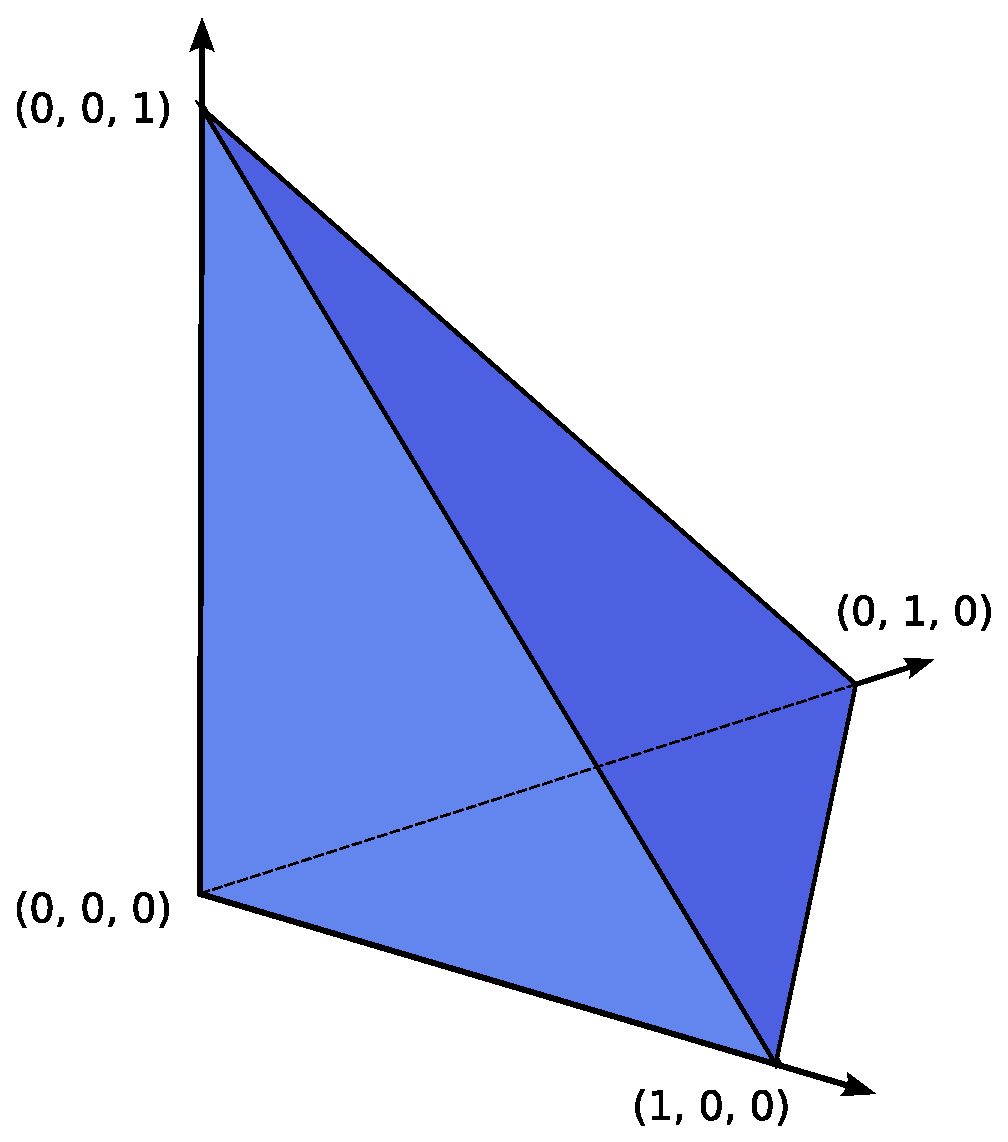
\includegraphics[width=10cm]{eps/tetrahedron.eps}
    \caption{The reference tetrahedron.}
  \end{center}
\end{figure}

\newpage
\section{The reference hexahedron}

\begin{figure}[H]
  \begin{center}
    \psfrag{v0}{$(0, 0, 0)$}
    \psfrag{v1}{$(1, 0, 0)$}
    \psfrag{v2}{$(1, 1, 0)$}
    \psfrag{v3}{$(0, 1, 0)$}
    \psfrag{v4}{$(0, 0, 1)$}
    \psfrag{v5}{$(1, 0, 1)$}
    \psfrag{v6}{$(1, 1, 1)$}
    \psfrag{v7}{$(0, 1, 1)$}
    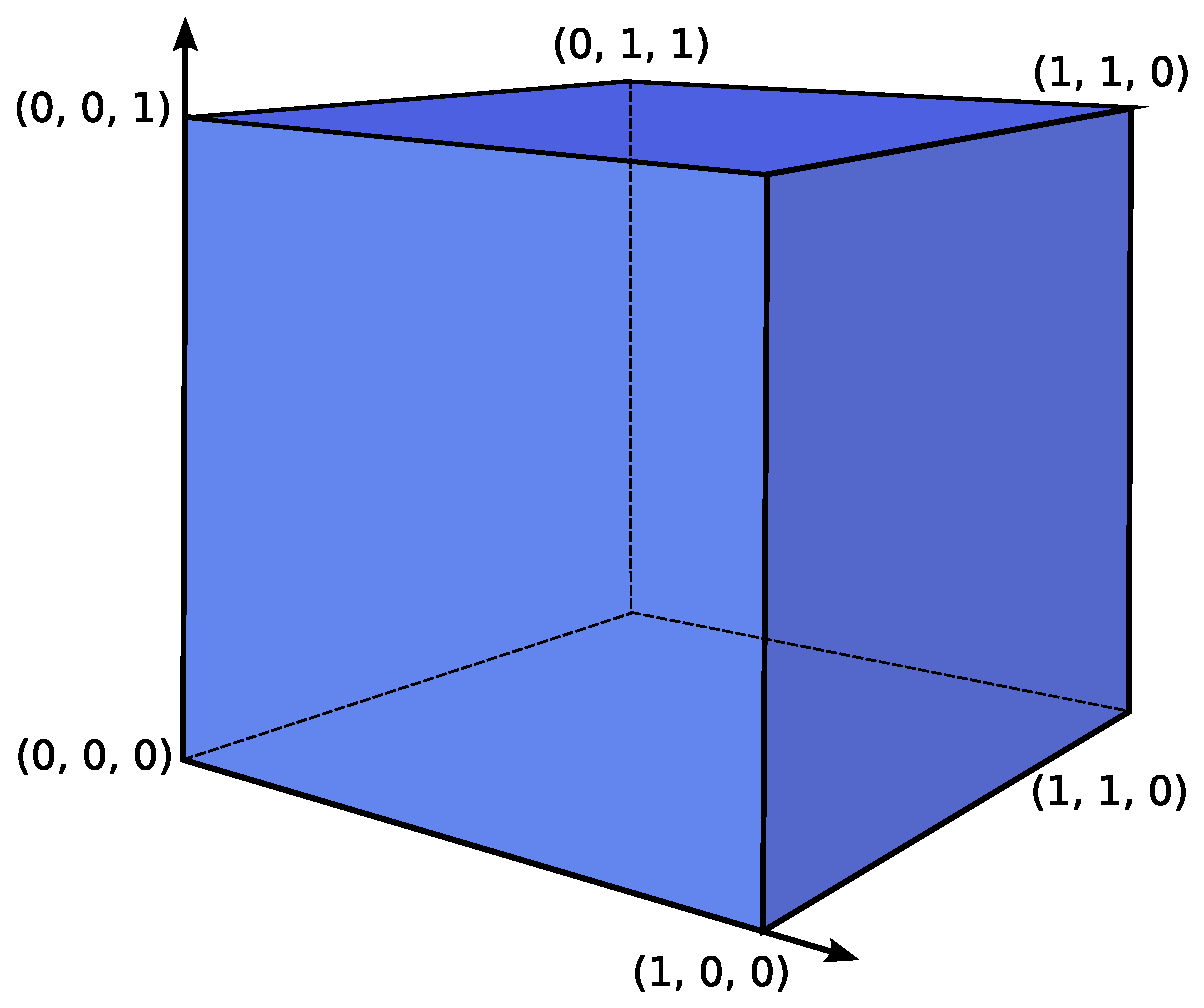
\includegraphics[width=10cm]{eps/hexahedron.eps}
    \caption{The reference hexahedron.}
  \end{center}
\end{figure}
